
\documentclass[letterpaper, reqno,11pt]{article}
\usepackage[margin=1.0in]{geometry}
\usepackage{color,latexsym,amsmath,amssymb}
\usepackage{fancyhdr}
\usepackage{amsthm}
\usepackage{mathtools}
\usepackage{tikz}
\usepackage{float}
\usepackage{centernot}
\usepackage{subcaption}
\usepackage{extarrows}
\usetikzlibrary{hobby}
\usetikzlibrary{shapes.multipart}
\usepackage{pgfplots}
\pgfplotsset{compat=1.7}
\usetikzlibrary{arrows.meta}
\usepackage{cancel}
\usetikzlibrary{decorations.markings}
\usetikzlibrary{shapes}
\usetikzlibrary{arrows}
\usepgfplotslibrary{fillbetween}
\usetikzlibrary{patterns}

\newcommand{\RR}{\mathbb{R}}
\newcommand{\CC}{\mathbb{C}}
\newcommand{\ZZ}{\mathbb{Z}}
\newcommand{\QQ}{\mathbb{Q}}
\newcommand{\NN}{\mathbb{N}}
\DeclareMathOperator{\id}{id}
\def\upint{\mathchoice%
  {\mkern13mu\overline{\vphantom{\intop}\mkern7mu}\mkern-20mu}%
  {\mkern7mu\overline{\vphantom{\intop}\mkern7mu}\mkern-14mu}%
  {\mkern7mu\overline{\vphantom{\intop}\mkern7mu}\mkern-14mu}%
  {\mkern7mu\overline{\vphantom{\intop}\mkern7mu}\mkern-14mu}%
  \int}
\def\lowint{\mkern3mu\underline{\vphantom{\intop}\mkern7mu}\mkern-10mu\int}
\DeclareMathOperator{\card}{card}
\DeclareMathOperator{\Binomial}{Binomial}
\DeclareMathOperator{\Span}{span}
\DeclareMathOperator{\sgn}{sgn}
\pagestyle{fancy}
\lhead{Math 321 Lecture 31}
\rhead{Yuchong Pan}
\begin{document}
\pagenumbering{arabic}
\title{Math 321 Lecture 31}
\author{Yuchong Pan}
\date{March 25, 2019}
\newtheorem{thm}{Theorem}
\newtheorem{defn}{Definition}
\newtheorem*{remark}{Remark}
\newtheorem{claim}{Claim}
\newtheorem{cor}{Corollary}
\newtheorem{lemma}{Lemma}
\newtheorem{prop}{Proposition}
\newtheorem{fact}{Fact}
\newtheorem{observation}{Observation}
\maketitle
%

\section{Proof of the Inverse Function Theorem (Cont'd)}

\begin{proof}[Proof (cont'd)]
  (b) {\bf Know:}
  \begin{itemize}
  \item $\mathbf f: \underbrace{U}_{\substack{\rotatebox[origin=c]{270}{$\subseteq$} \\ E \\ \rotatebox[origin=c]{270}{$\subseteq$} \\ \RR^n}} \xrightarrow{\text{bijection}} \mathbf f(U) = V \subseteq \RR^n$ from part (a).
  \item $\mathbf a \in U \subseteq E$.
  \item $\mathbf g = \mathbf f^{-1} : V \to U$.
  \end{itemize}
  
  \noindent {\bf Goal:} $\mathbf g$ is $C^1$.

  \medskip

  Let
  \begin{align*}
    \mathbf g(\mathbf y + \mathbf k) = \mathbf x + \mathbf h \quad &\Leftrightarrow \quad \mathbf f(\mathbf x + \mathbf h) = \mathbf y + \mathbf k, && \mathbf x \in U, \quad \mathbf y \in V. \\
    \mathbf g(\mathbf y) = \mathbf x \quad &\Leftrightarrow \quad \mathbf f(\mathbf x) = \mathbf y.
  \end{align*}
  We have shown that
  \begin{gather*}
    \mathbf A = \mathbf f'(\mathbf a) \text{ invertible} \\
    \Downarrow \\
    \mathbf f'(x) \text{ invertible for } \underbrace{\text{$\mathbf x$ near $\mathbf a$}}_\text{so for $\mathbf x \in U$} \\
    \Downarrow \\
    \mathbf T = (\mathbf f'(\mathbf x))^{-1} \text{ well-defined}.
  \end{gather*}
  Hence,
  \begin{align*}
    & \text{$\mathbf g$ is differentiable at $\mathbf y$ with the derivative $\mathbf T = (\mathbf f(\mathbf x))^{-1}$} \\
    \Leftrightarrow \quad & \mathcal A = \boxed{\frac{\lVert \overbrace{\mathbf g(\mathbf y + \mathbf k)}^{= \mathbf x + \mathbf h} - \overbrace{\mathbf g(\mathbf y)}^{= \mathbf x} - \overbrace{\mathbf T}^{= (\mathbf f'(\mathbf x))^{-1}} \mathbf k \rVert}{\lVert \mathbf k \rVert}} \xrightarrow{k \to 0} 0.
  \end{align*}
  We have
  \begin{align*}
    \mathcal A &= \frac{\lVert (\cancel{\mathbf x} + \mathbf h) - \cancel{\mathbf x} - (\mathbf f'(\mathbf x))^{-1} (\mathbf f(\mathbf x + \mathbf h) - \mathbf f(\mathbf x)) \rVert}{\lVert \mathbf k \rVert} \\
    &= \frac{\lVert \overbrace{\mathbf h}^{= \mathbf I \mathbf h = (\mathbf f'(\mathbf x))^{-1} (\mathbf f'(\mathbf x)) \mathbf h} - (\mathbf f'(\mathbf x))^{-1} (\mathbf f(\mathbf x + \mathbf h) - \mathbf f(\mathbf x)) \rVert}{\lVert \mathbf k \rVert} \\
    &= \frac{\lVert (\mathbf f'(\mathbf x))^{-1} (\mathbf f'(\mathbf x) \mathbf h - (\mathbf f(\mathbf x + \mathbf h) - \mathbf f(\mathbf x))) \rVert}{\lVert \mathbf k \rVert} \\
    & \leq \underbrace{\frac{\lVert (\mathbf f'(\mathbf x))^{-1} \rVert}{\lVert \mathbf k \rVert} \lVert \mathbf h \rVert}_\text{we need to show this stays bounded} \underbrace{\frac{\lVert \mathbf f(\mathbf x + \mathbf h) - \mathbf f(\mathbf x) - \mathbf f'(\mathbf x) \mathbf h \rVert}{\lVert \mathbf h \rVert}}_{\substack{\text{$\to 0$ as $\mathbf h \to \mathbf 0 \Leftrightarrow \mathbf k \to \mathbf 0$ } \\ \text{because $\mathbf f$ is differentiable at $\mathbf x$}}}.
  \end{align*}

  \begin{observation}
    \normalfont $\mathbf f'(\mathbf x)$ is closed to $\mathbf f'(\mathbf a)$ if $\mathbf x$ is close to $\mathbf a$ because $\underbrace{\mathbf f \in C^1(E)}_\text{$x \mapsto \mathbf f'(x)$ continuous}$.
  \end{observation}
  
  \noindent This implies that $\left\lVert (\mathbf f'(\mathbf x))^{-1} \right\rVert$ is bounded from above for $\mathbf x \in U$, where $\lVert \mathbf A \rVert = \sup_{\mathbf x \neq \mathbf 0} \frac{\lVert \mathbf A \mathbf x \rVert}{\lVert \mathbf x \rVert}$ for an $m \times n$ matrix $\mathbf A$.

  \medskip

  \noindent {\bf Recall from (a):} $\varphi_{\mathbf y} (\mathbf x) = \mathbf x + \mathbf A^{-1} (\mathbf y - \mathbf f(\mathbf x))$ is a contraction for $\mathbf x \in U$; more precisely,
  \begin{align*}
    & \lVert \varphi_{\mathbf y}(\underbrace{\mathbf x_1}_{= \mathbf x + \mathbf h}) - \varphi_{\mathbf y}(\underbrace{\mathbf x_2}_{= \mathbf x}) \rVert < \frac{1}{2} \lVert \underbrace{\mathbf x_1 - \mathbf x_2}_{\mathbf h} \rVert && \mathbf x_1, x_2 \in U \\
    \Rightarrow \quad & \lVert \cancel{\mathbf x} + \mathbf h + \mathbf A^{-1} (\cancel{\mathbf y} - \mathbf f(\mathbf x + \mathbf h)) - (\cancel{\mathbf x} + \mathbf A^{-1}(\cancel{\mathbf y} - \mathbf f(\mathbf x))) \rVert < \frac{1}{2} \lVert \mathbf h \rVert.
  \end{align*}
  So,
  \[ \lVert \mathbf h - \mathbf A^{-1}(\underbrace{\mathbf f(\mathbf x + \mathbf h)}_{\mathbf y + \mathbf k} - \underbrace{\mathbf f(\mathbf x))}_{\mathbf y} \rVert < \frac{1}{2} \lVert \mathbf h \rVert. \]
  This implies that
  \begin{align*}
    \lVert \mathbf h - \mathbf A^{-1} \mathbf k \rVert < \frac{1}{2} \lVert \mathbf h \rVert \quad \Rightarrow \quad \underbrace{\lVert \mathbf A^{-1} \mathbf k \rVert}_{\substack{\rotatebox[origin=c]{270}{$\leq$} \\ \lVert A^{-1} \rVert \cdot \lVert \mathbf k \rVert}} &\geq \lVert \mathbf h \rVert - \lVert \mathbf h - \mathbf A^{-1} \mathbf k \rVert && \text{reverse triangle inequality} \\
    &\geq \lVert \mathbf h \rVert - \frac{1}{2} \lVert \mathbf h \rVert \\
    &= \frac{\lVert \mathbf h \rVert}{2}.
  \end{align*}

  \noindent {\bf Get:} $\frac{\lVert \mathbf h \rVert}{2} \leq \lVert \mathbf A^{-1} \rVert \cdot \lVert \mathbf k \rVert$; i.e., $\frac{\lVert \mathbf h \rVert}{\lVert \mathbf k \rVert} \leq 2 \cdot \lVert \mathbf A^{-1} \rVert$; i.e., as $\mathbf h, \mathbf k \to 0$, $\frac{\lVert \mathbf h \rVert}{\lVert \mathbf k \rVert}$ stays bounded.

  \begin{figure}[H]
    \centering
    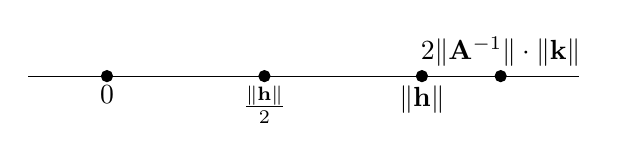
\begin{tikzpicture}
      \draw (0, 0) -- (7, 0);
      \draw[fill=black] (1, 0) circle (2pt) node[below] {$0$};
      \draw[fill=black] (3, 0) circle (2pt) node[below] {$\frac{\lVert \mathbf h \rVert}{2}$};
      \draw[fill=black] (5, 0) circle (2pt) node[below] {$\lVert \mathbf h \rVert$};
      \draw[fill=black] (6, 0) circle (2pt) node[above] {$2 \lVert \mathbf A^{-1} \rVert \cdot \lVert \mathbf k \rVert$};
    \end{tikzpicture}
  \end{figure}
\end{proof}

\noindent {\bf Proof overview:}
\begin{enumerate}
\item Show $\mathbf f$ is locally bijective. Find $U = B(\mathbf a; \epsilon)$.
  \begin{enumerate}
  \item $V = \mathbf f(U)$: $\mathbf f$ surjective.
  \item CMP used to prove $\mathbf f$ injective.
  \item {\bf Exercise:} $V$ is open.
  \end{enumerate}
\item Relate $\mathbf g'$ with $\mathbf f'$ where $\mathbf g = \mathbf f^{-1}$.
  \[ \mathbf g'(\mathbf y) = \mathbf g'(\mathbf f(\mathbf x)) = (\mathbf f'(\mathbf x))^{-1}. \]
  \noindent {\bf Critical:} $\begin{array}{l}
      \lVert \mathbf h \rVert \to 0 \\
      \lVert \mathbf k \rVert \to 0
  \end{array}$ at comparable rates; i.e., $\frac{\lVert \mathbf h \rVert}{\lVert \mathbf k \rVert}$ stays bounded.
\end{enumerate}

\section{Implicit Function Theorem}

\noindent {\bf Question:} Given any equation $f(x, y) = 0$ where $f : \RR^2 \to \RR$, when can we solve it to get $y = g(x)$?

\begin{remark}
  \normalfont ~
  \begin{enumerate}
  \item For arbitrarily chosen $f$, no guarantee of any solution; e.g., $f(x, y) = x^2 + y^2 + 1$. Need to assume $(a, b) \in \RR^2$ such that $f(a, b) = 0$.
  \item Suppose such $(a, b)$ exists. Does this always imply that for \emph{every} $x$ in a neighbourhood of $a$, one can find $y = g(x)$ such that $f(x, g(x)) = 0$?

    \noindent {\bf Answer:} No.

    \noindent {\bf Examples:}
    \begin{enumerate}
    \item $f(x, y) = x^2 + y^2, (a, b) = (0, 0)$. No other solution exists for $x \neq a$.
    \item $f(x, y) = x^2 + y^2 - 1$.
    \end{enumerate}

    \begin{figure}[H]
      \centering
      \begin{tikzpicture}
        \draw[->] (-3, 0) -- (3, 0);
        \draw[->] (0, -3) -- (0, 3);
        \draw[blue] (0, 0) circle (2);
        \draw (1.5, -1.323) -- (1.5, 1.323);
        \node[below left] at (1.5, 0) {$x$};
        \node[above right] at (1.5, 1.323) {$g(x)$};
        \node[below right] at (1.5, -1.323) {$g'(x)$};
      \end{tikzpicture}
    \end{figure}
  \end{enumerate}
\end{remark}

\end{document}
